\documentclass[12pt]{article}
\usepackage{amsmath}
\usepackage{graphicx}
\usepackage{tikz}
\usepackage{pgfplots}
\usetikzlibrary{shapes,arrows}
\usepgfplotslibrary{fillbetween}


\title{Algebraic Inequalities}\\
\author{Tutoring Centre Ferndale\\

\includegraphics[width=4em]{ApS_logo.png}}
\date{}

\begin{document}

\maketitle

Algebraic inequalities are statements that compare two expressions using inequality symbols. They are used to show the relationship between quantities that are not necessarily equal.

\section*{Inequality Symbols}

\begin{itemize}
    \item \( < \): less than
    \item \( \leq \): less than or equal to
    \item \( > \): greater than
    \item \( \geq \): greater than or equal to
\end{itemize}

\section*{Rules for Solving Inequalities}

\begin{itemize}
    \item \textbf{Addition/Subtraction Rule}: You can add or subtract the same number from both sides of an inequality without changing its direction.
    \item \textbf{Multiplication/Division Rule}: You can multiply or divide both sides of an inequality by the same positive number without changing its direction. If you multiply or divide by a negative number, you must reverse the direction of the inequality.
\end{itemize}

\section*{Examples}

\subsection*{Example 1}

Solve \( x + 3 < 7 \).

\begin{itemize}
    \item Subtract 3 from both sides: \( x < 4 \).
\end{itemize}

\subsection*{Example 2}

Solve \( 2x \geq 10 \).

\begin{itemize}
    \item Divide both sides by 2: \( x \geq 5 \).
\end{itemize}

\subsection*{Example 3}

Solve \( -3x < 9 \).

\begin{itemize}
    \item Divide both sides by -3 and reverse the inequality: \( x > -3 \).
\end{itemize}

\section*{Graphing Inequalities}

Graphing inequalities on a number line helps to visualize the solution set.

\subsection*{Example 4}

Graph \( x < 4 \).

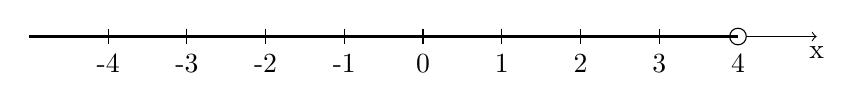
\begin{tikzpicture}
    \draw[->] (-5,0) -- (5,0) node[anchor=north] {x};
    \foreach \x in {-4,-3,...,4}
        \draw (\x,0.1) -- (\x,-0.1) node[anchor=north] {\x};
    \draw[fill=white] (4,0) circle (3pt);
    \draw[very thick] (-5,0) -- (4,0);
\end{tikzpicture}

\subsection*{Example 5}

Graph \( x \geq -2 \).

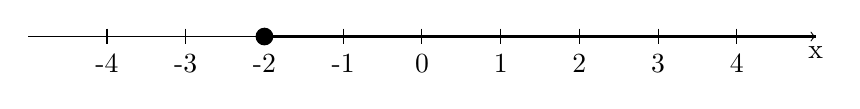
\begin{tikzpicture}
    \draw[->] (-5,0) -- (5,0) node[anchor=north] {x};
    \foreach \x in {-4,-3,...,4}
        \draw (\x,0.1) -- (\x,-0.1) node[anchor=north] {\x};
    \draw[fill=black] (-2,0) circle (3pt);
    \draw[very thick] (-2,0) -- (5,0);
\end{tikzpicture}

\subsection*{Example 6: Quadratic Inequality}

Solve and graph the inequality \( y < x^2 - 2x + 1 \).

\begin{itemize}
    \item This inequality represents the region below the parabola defined by the equation \( y = x^2 - 2x + 1 \).
\end{itemize}

Graph:

\begin{center}
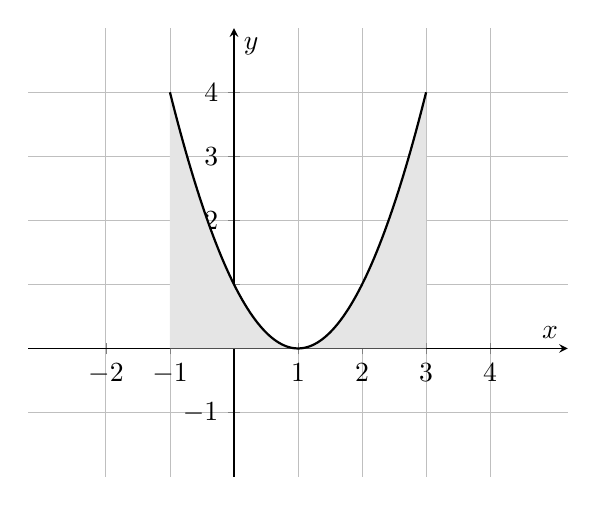
\begin{tikzpicture}
\begin{axis}[
    axis lines = middle,
    xlabel = {$x$},
    ylabel = {$y$},
    domain=-1:3,
    xmin=-1, xmax=3,
    ymin=-2, ymax=5,
    samples=100,
    clip=false,
    ytick={-1,0,1,2,3,4},
    xtick={-2,-1,0,1,2,3,4},
    grid=both,
    grid style={line width=.3pt, draw=gray!50},
    axis equal
]
\addplot [fill=gray!20,draw=none,domain=-1:3]
    {x^2 - 2*x + 1} \closedcycle;
\addplot [thick, domain=-1:3]
    {x^2 - 2*x + 1};
\end{axis}
\end{tikzpicture}
\end{center}

\section*{Exercises}

\subsection*{Exercise 1}

Solve and graph the inequality \( x - 5 \leq 2 \).

\subsection*{Exercise 2}

Solve and graph the inequality \( 4x > 12 \).

\subsection*{Exercise 3}

Solve and graph the inequality \( -2x \geq 6 \).

\subsection*{Exercise 4}

Graph the inequality \( y \leq 2x+1 \).

\section*{Answers}

\subsection*{Answer 1}

Solve \( x - 5 \leq 2 \).

\begin{itemize}
    \item Add 5 to both sides: \( x \leq 7 \).
\end{itemize}

Graph:

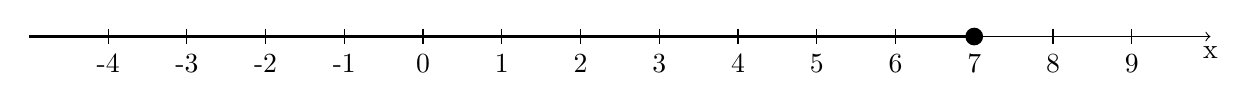
\begin{tikzpicture}
    \draw[->] (-5,0) -- (10,0) node[anchor=north] {x};
    \foreach \x in {-4,-3,...,9}
        \draw (\x,0.1) -- (\x,-0.1) node[anchor=north] {\x};
    \draw[fill=black] (7,0) circle (3pt);
    \draw[very thick] (-5,0) -- (7,0);
\end{tikzpicture}

\subsection*{Answer 2}

Solve \( 4x > 12 \).

\begin{itemize}
    \item Divide both sides by 4: \( x > 3 \).
\end{itemize}

Graph:

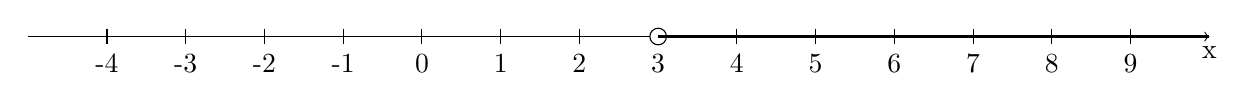
\begin{tikzpicture}
    \draw[->] (-5,0) -- (10,0) node[anchor=north] {x};
    \foreach \x in {-4,-3,...,9}
        \draw (\x,0.1) -- (\x,-0.1) node[anchor=north] {\x};
    \draw[fill=white] (3,0) circle (3pt);
    \draw[very thick] (3,0) -- (10,0);
\end{tikzpicture}

\subsection*{Answer 3}

Solve \( -2x \geq 6 \).

\begin{itemize}
    \item Divide both sides by -2 and reverse the inequality: \( x \leq -3 \).
\end{itemize}

Graph:

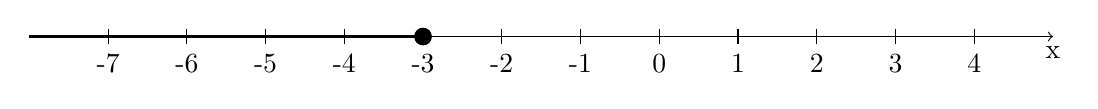
\begin{tikzpicture}
    \draw[->] (-8,0) -- (5,0) node[anchor=north] {x};
    \foreach \x in {-7,-6,...,4}
        \draw (\x,0.1) -- (\x,-0.1) node[anchor=north] {\x};
    \draw[fill=black] (-3,0) circle (3pt);
    \draw[very thick] (-8,0) -- (-3,0);
\end{tikzpicture}

\newpage

\subsection*{Answer 4}

Graph: $y\leq2x+1$

\begin{center}
\begin{tikzpicture}
\begin{axis}[width=\textwidth,
    axis lines = middle,
    xlabel = {$x$},
    ylabel = {$y$},
    domain=-1:4,
    xmin=-2, xmax=5,
    ymin=-2, ymax=10,
    samples=100,
    clip=false,
    ytick={-2,-1,0,1,2,3,4,5,6,7,8,9,10},
    xtick={-2, -1, 0, 1, 2, 3, 4, 5},
    grid=both,
    grid style={line width=.3pt, draw=gray!50},
    axis equal
]
\addplot [fill=gray!20,draw=none,domain=-1:4]
    {2*x + 1} \closedcycle -10;
\addplot [<->,thick, domain=-1:4]
    {2*x + 1};
\end{axis}
\end{tikzpicture}
\end{center}

\end{document}
